\PassOptionsToPackage{unicode=true}{hyperref} % options for packages loaded elsewhere
\PassOptionsToPackage{hyphens}{url}
%
\documentclass[ignorenonframetext,]{beamer}
\usepackage{pgfpages}
\setbeamertemplate{caption}[numbered]
\setbeamertemplate{caption label separator}{: }
\setbeamercolor{caption name}{fg=normal text.fg}
\beamertemplatenavigationsymbolsempty
% Prevent slide breaks in the middle of a paragraph:
\widowpenalties 1 10000
\raggedbottom
\setbeamertemplate{part page}{
\centering
\begin{beamercolorbox}[sep=16pt,center]{part title}
  \usebeamerfont{part title}\insertpart\par
\end{beamercolorbox}
}
\setbeamertemplate{section page}{
\centering
\begin{beamercolorbox}[sep=12pt,center]{part title}
  \usebeamerfont{section title}\insertsection\par
\end{beamercolorbox}
}
\setbeamertemplate{subsection page}{
\centering
\begin{beamercolorbox}[sep=8pt,center]{part title}
  \usebeamerfont{subsection title}\insertsubsection\par
\end{beamercolorbox}
}
\AtBeginPart{
  \frame{\partpage}
}
\AtBeginSection{
  \ifbibliography
  \else
    \frame{\sectionpage}
  \fi
}
\AtBeginSubsection{
  \frame{\subsectionpage}
}
\usepackage{lmodern}
\usepackage{amssymb,amsmath}
\usepackage{ifxetex,ifluatex}
\usepackage{fixltx2e} % provides \textsubscript
\ifnum 0\ifxetex 1\fi\ifluatex 1\fi=0 % if pdftex
  \usepackage[T1]{fontenc}
  \usepackage[utf8]{inputenc}
  \usepackage{textcomp} % provides euro and other symbols
\else % if luatex or xelatex
  \usepackage{unicode-math}
  \defaultfontfeatures{Ligatures=TeX,Scale=MatchLowercase}
\fi
% use upquote if available, for straight quotes in verbatim environments
\IfFileExists{upquote.sty}{\usepackage{upquote}}{}
% use microtype if available
\IfFileExists{microtype.sty}{%
\usepackage[]{microtype}
\UseMicrotypeSet[protrusion]{basicmath} % disable protrusion for tt fonts
}{}
\IfFileExists{parskip.sty}{%
\usepackage{parskip}
}{% else
\setlength{\parindent}{0pt}
\setlength{\parskip}{6pt plus 2pt minus 1pt}
}
\usepackage{hyperref}
\hypersetup{
            pdftitle={Einführung R},
            pdfauthor={Jan-Philipp Kolb},
            pdfborder={0 0 0},
            breaklinks=true}
\urlstyle{same}  % don't use monospace font for urls
\newif\ifbibliography
\usepackage{graphicx,grffile}
\makeatletter
\def\maxwidth{\ifdim\Gin@nat@width>\linewidth\linewidth\else\Gin@nat@width\fi}
\def\maxheight{\ifdim\Gin@nat@height>\textheight\textheight\else\Gin@nat@height\fi}
\makeatother
% Scale images if necessary, so that they will not overflow the page
% margins by default, and it is still possible to overwrite the defaults
% using explicit options in \includegraphics[width, height, ...]{}
\setkeys{Gin}{width=\maxwidth,height=\maxheight,keepaspectratio}
\setlength{\emergencystretch}{3em}  % prevent overfull lines
\providecommand{\tightlist}{%
  \setlength{\itemsep}{0pt}\setlength{\parskip}{0pt}}
\setcounter{secnumdepth}{0}

% set default figure placement to htbp
\makeatletter
\def\fps@figure{htbp}
\makeatother


\title{Einführung R}
\author{Jan-Philipp Kolb}
\date{7 Januar 2019}

\begin{document}
\frame{\titlepage}

\begin{frame}{Gründe R zu nutzen\ldots{}}
\protect\hypertarget{grunde-r-zu-nutzen}{}

\begin{itemize}
\item
  \ldots{} R ist eine
  \href{https://stackoverflow.com/questions/1546583/what-is-the-definition-of-an-open-source-programming-language}{\textbf{quelloffene
  Sprache}}
\item
  \ldots{} hervorragende
  \href{http://matthewlincoln.net/2014/12/20/adjacency-matrix-plots-with-r-and-ggplot2.html}{\textbf{Grafiken}},
  \href{https://www.r-bloggers.com/3d-plots-with-ggplot2-and-plotly\%20/}{\textbf{Grafiken}},
  \href{https://procomun.wordpress.com/2011/03/18/splomr/}{\textbf{Grafiken}}
\item
  \ldots{} \href{https://github.com/Japhilko/RInterfaces}{\textbf{R kann
  in Kombination mit anderen Programmen verwendet werden}} - z.B. zur
  \href{https://github.com/Japhilko/RInterfaces/blob/master/slides/Datenimport.md}{\textbf{Verknüpfung
  von Daten}}
\item
  \ldots{} R kann
  \href{https://cran.r-project.org/web/packages/MplusAutomation/index.html}{\textbf{zur
  Automatisierung}} verwendet werden
\item
  \ldots{} Breite und aktive Community -
  \href{https://www.r-bloggers.com/}{\textbf{Man kann die Intelligenz
  anderer Leute nutzen ;-)}}
\end{itemize}

\end{frame}

\begin{frame}{R kann in Kombination mit anderen Programmen genutzt
werden\ldots{}}
\protect\hypertarget{r-kann-in-kombination-mit-anderen-programmen-genutzt-werden}{}

\begin{figure}
\centering
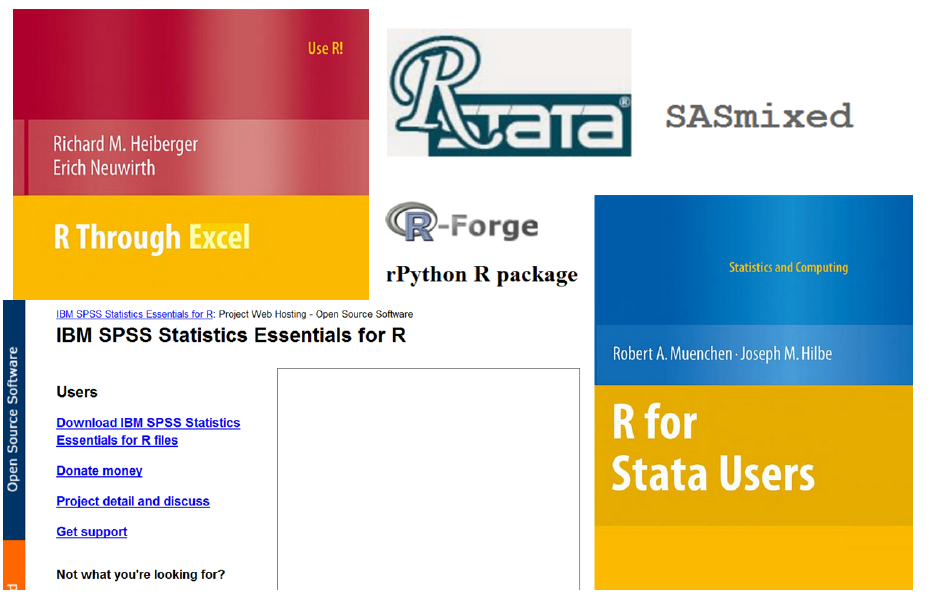
\includegraphics{D:/Daten/GitHub/IntroR/buildingblocks/figure/Rinterfaces.PNG}
\caption{Schnittstellen zu R}
\end{figure}

\begin{itemize}
\tightlist
\item
  Schnittstelle zu:
  \href{https://cran.r-project.org/web/packages/reticulate/vignettes/calling_python.html}{\textbf{Python}},
  \href{https://www.springer.com/de/book/9781441900517}{\textbf{Excel}},
  \href{https://www.ibm.com/support/knowledgecenter/en/SSFUEU_7.2.0/com.ibm.swg.ba.cognos.op_capmod_ig.7.2.0.doc/t_essentials_for_r_statistics.html}{\textbf{SPSS}},
  \href{https://cran.r-project.org/web/packages/SASmixed/index.html}{\textbf{SAS}},
  \href{https://cran.r-project.org/web/packages/RStata/index.html}{\textbf{Stata}}
\end{itemize}

\end{frame}

\begin{frame}{\href{https://gallery.shinyapps.io/cran-gauge/}{\textbf{Die
Beliebtheit von R-Paketen}}}
\protect\hypertarget{die-beliebtheit-von-r-paketen}{}

\begin{figure}
\centering
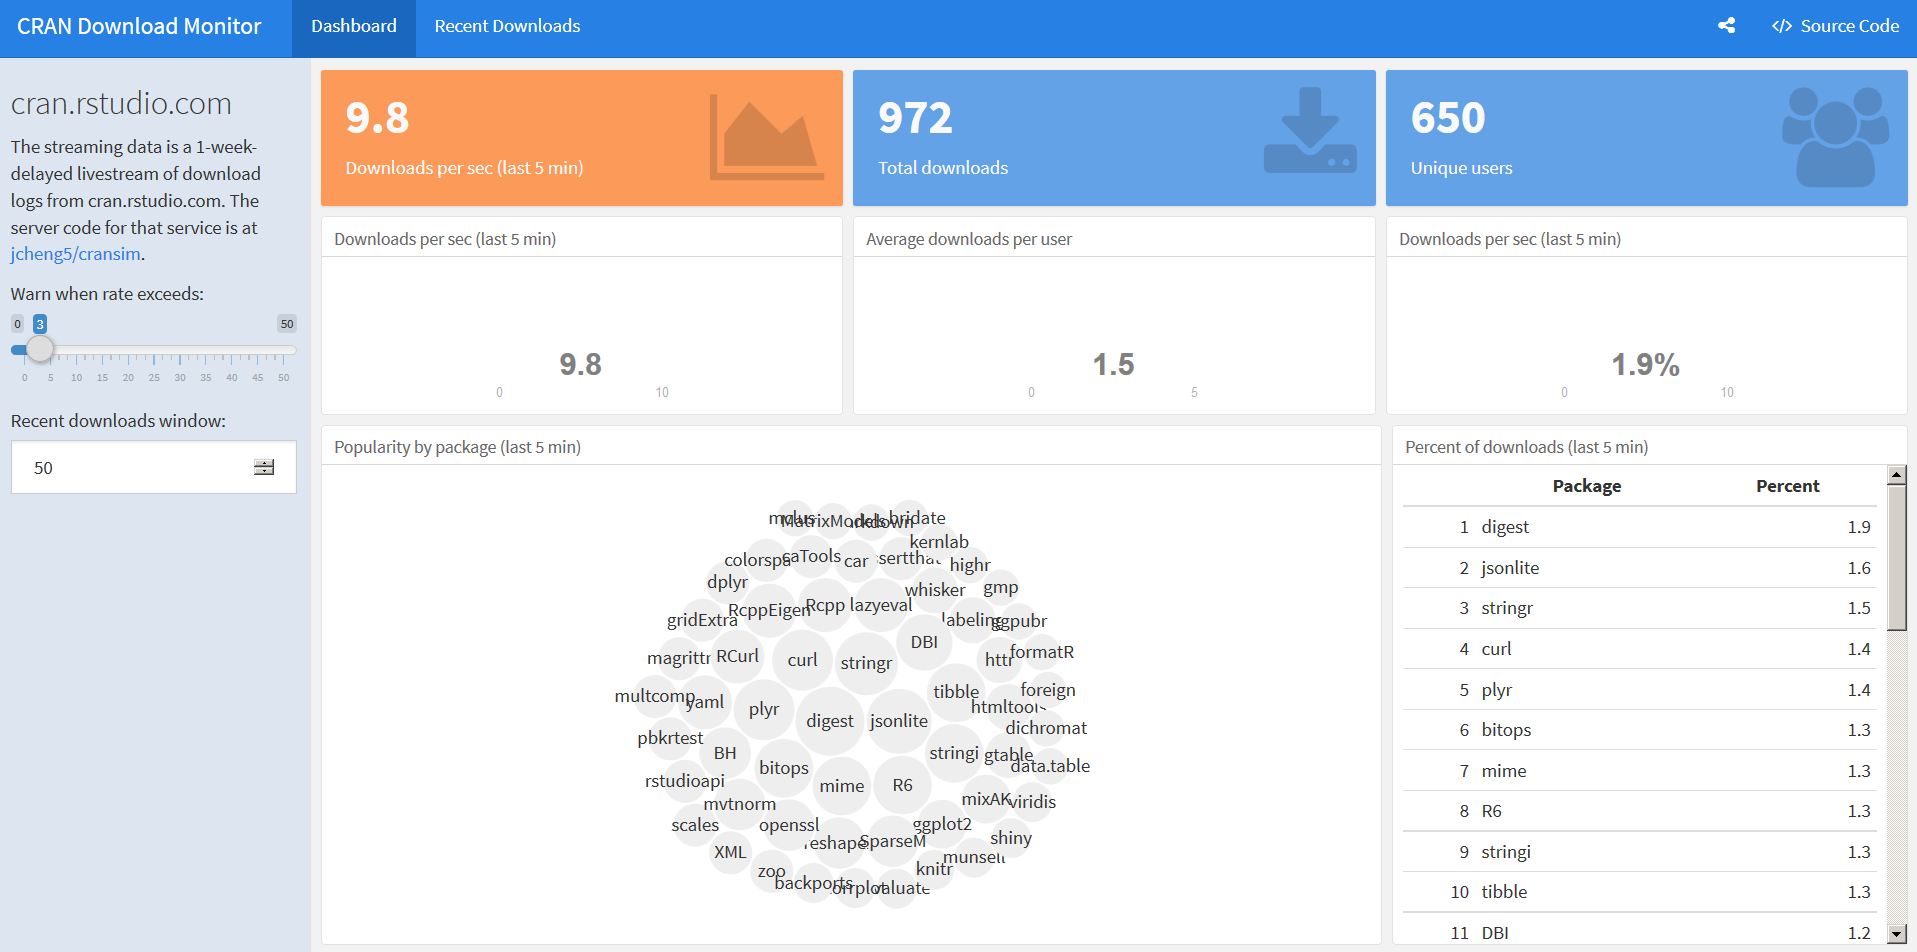
\includegraphics{D:/Daten/GitHub/IntroR/buildingblocks/figure/CRANdownloads.PNG}
\caption{Downloads vom CRAN Server}
\end{figure}

\end{frame}

\begin{frame}{Download R:}
\protect\hypertarget{download-r}{}

\url{http://www.r-project.org/}

\begin{figure}
\centering
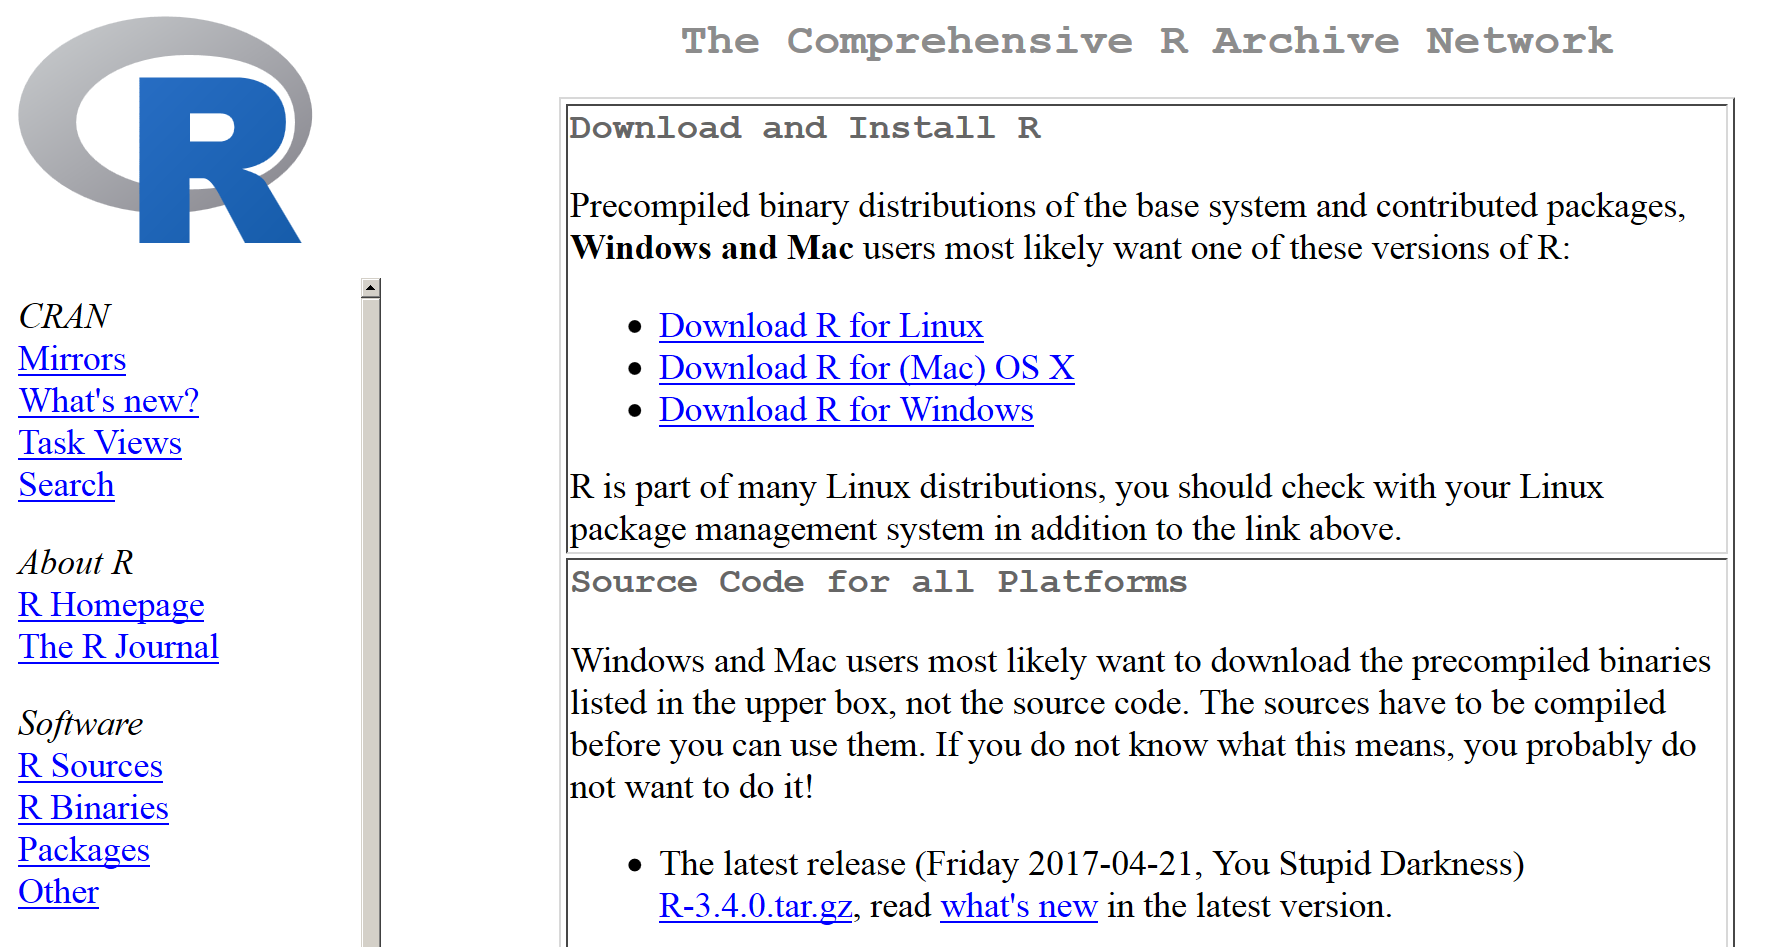
\includegraphics{D:/Daten/GitHub/IntroR/buildingblocks/figure/CRAN1picture.PNG}
\caption{The CRAN website}
\end{figure}

\end{frame}

\begin{frame}{Open Source Programm R}
\protect\hypertarget{open-source-programm-r}{}

\begin{block}{Das ist das Basis-R:}

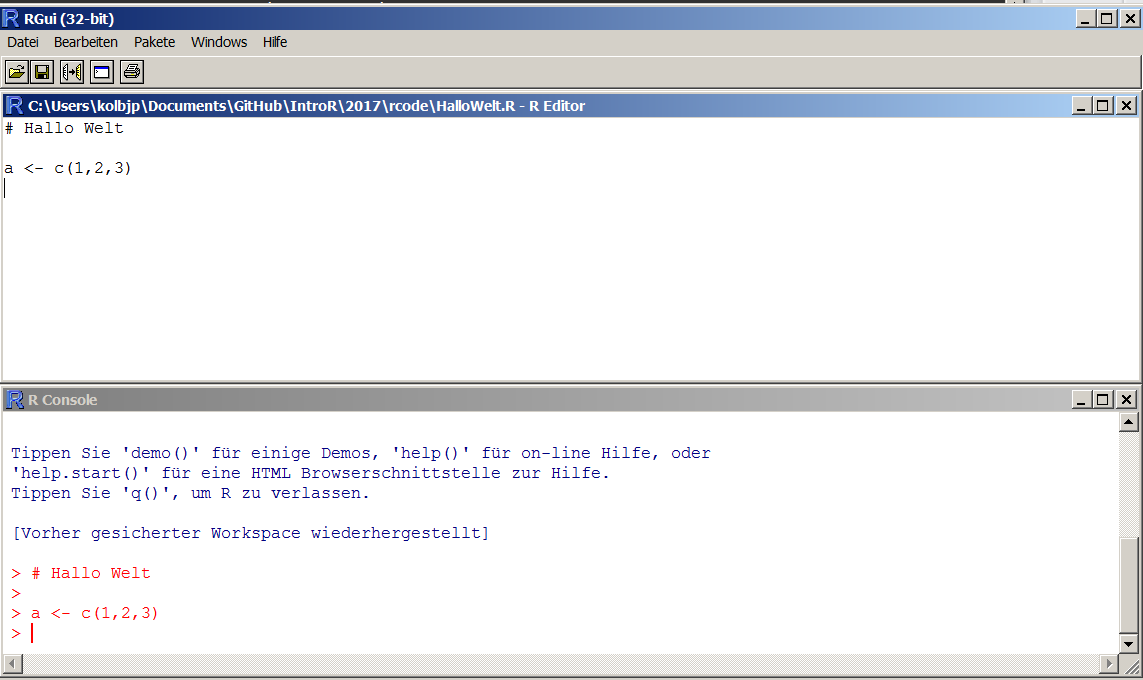
\includegraphics{D:/Daten/GitHub/IntroR/buildingblocks/figure/BasisR.PNG}

\end{block}

\end{frame}

\begin{frame}{Graphical user interface}
\protect\hypertarget{graphical-user-interface}{}

Viele Leute nutzen ein
\href{https://en.wikipedia.org/wiki/Graphical_user_interface}{\textbf{Graphical
User Interface}} (GUI) oder ein
\href{https://en.wikipedia.org/wiki/Integrated_development_environment}{\textbf{Integrated
Development Interface}} (IDE).

Aus den folgenden Gründen:

\begin{itemize}
\tightlist
\item
  Syntax-Hervorhebung
\item
  Auto-Vervollständigung
\item
  Bessere Übersicht über Graphiken, Pakete, Dateien, \ldots{}
\end{itemize}

\end{frame}

\begin{frame}{RStudio}
\protect\hypertarget{rstudio}{}

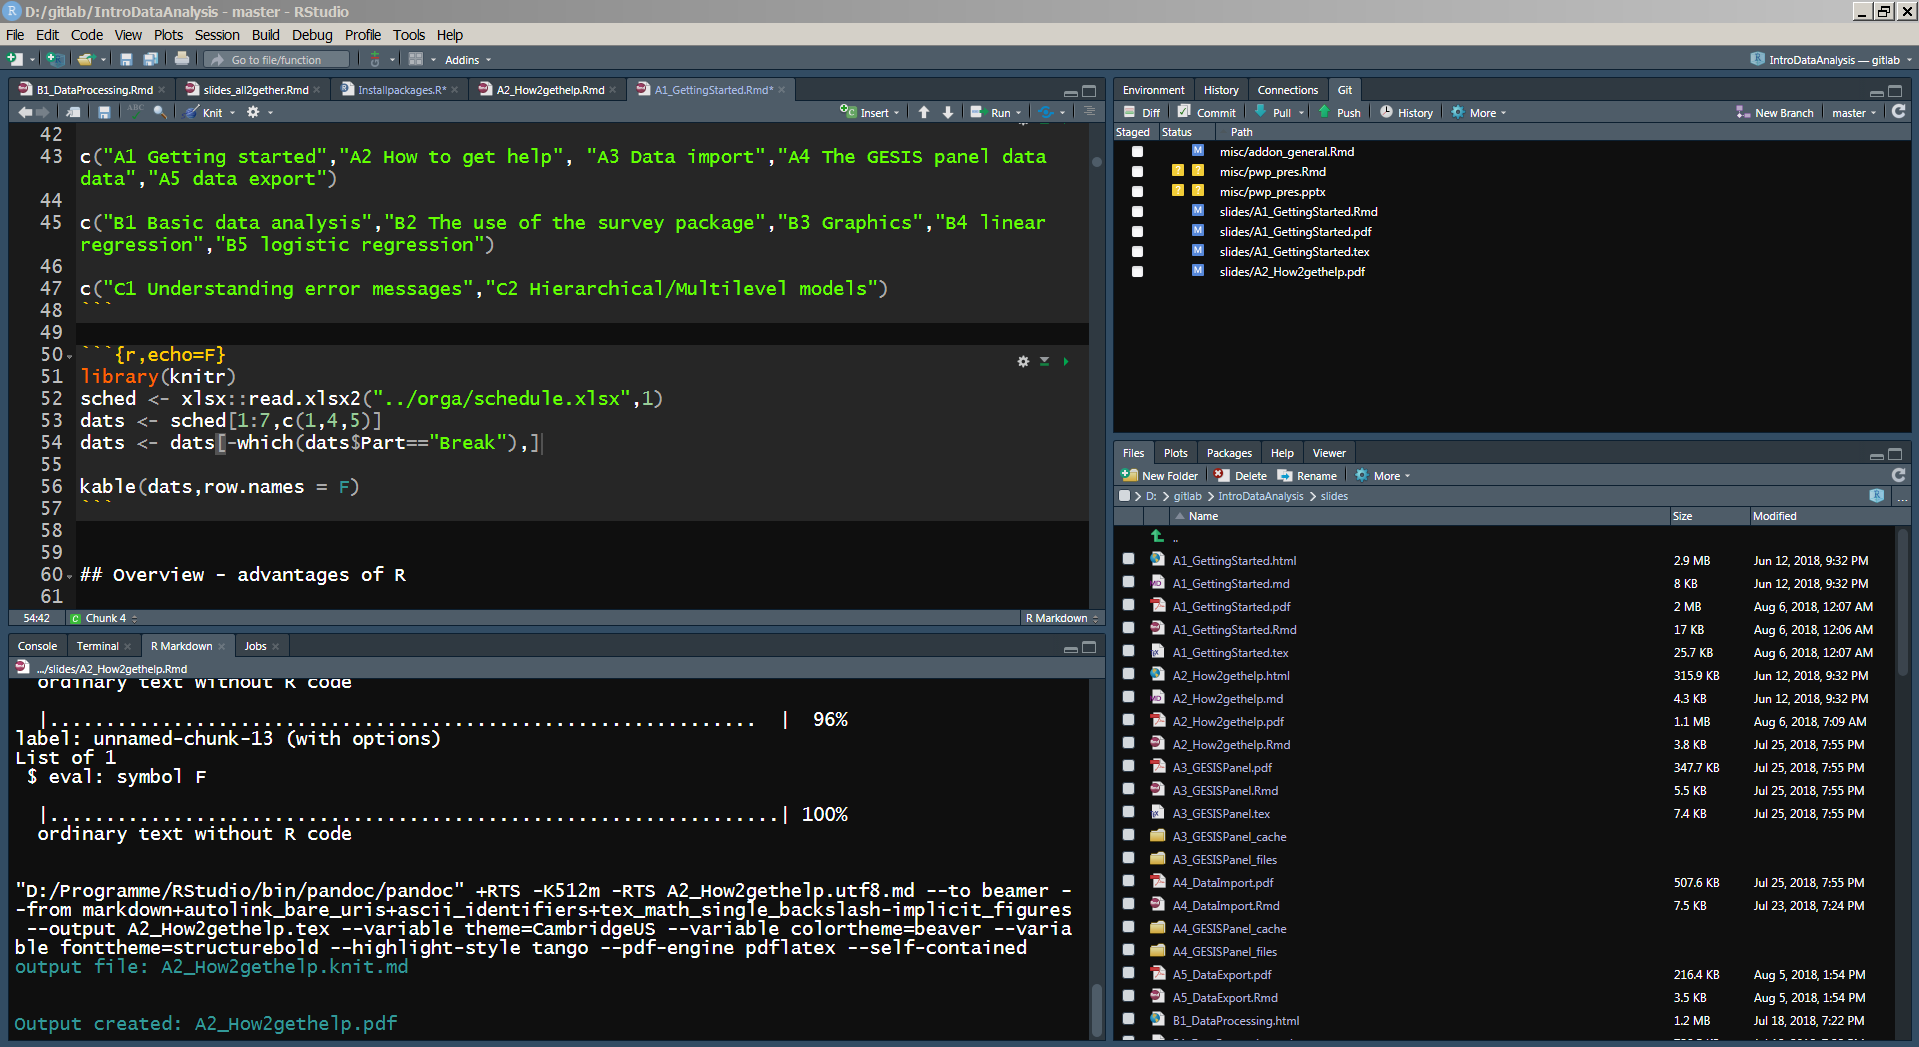
\includegraphics{D:/Daten/GitHub/IntroR/buildingblocks/figure/RstudioExample.PNG}

\end{frame}

\begin{frame}[fragile]{Übung - Vorbereitung}
\protect\hypertarget{ubung---vorbereitung}{}

\begin{itemize}
\item
  Schaue, ob R auf dem Computer installiert ist
\item
  Wenn nicht, lade \href{r-project.org}{\textbf{R}} herunter und
  installiere es.
\item
  Prüfe ob Rstudio installiert ist.
\item
  Wenn nicht - \href{http://www.rstudio.com/}{\textbf{installiere}}
  Rstudio.
\item
  Starte RStudio. Gehe in die Konsole (meistens Fenster unten links) und
  tippe
\item
  Wenn noch kein Skript geöffnet im oberen linken Teil von Rstudio
  geöffnet ist, gehe zum Menü und öffne ein neues Skript. Checks das
  Datum mit \texttt{date()} und die R version mit
  \texttt{sessionInfo()}.
\end{itemize}

\end{frame}

\end{document}
